%!TEX root=../document.tex

\section{Ergebnisse}
\subsection{Klasse Bruch}
Die Klasse Bruch soll Bruchteile darstellen können. Sie implementiert fast alle von Python bereitgestellten magischen Methoden, dadurch kann man sehr angenehm mit dieser Klasse arbeiten. 

\subsection{Beispiele} 
\begin{lstlisting}[language=Python]
print(Bruch(5,4))
\end{lstlisting}
Output: \verb|(5/4)|
\\\\


\begin{lstlisting}[language=Python]
print(float(Bruch(5,4)))
\end{lstlisting}
Output: \verb|1,25|
\\\\


\begin{lstlisting}[language=Python]
print(Bruch(3,2) + 1)
\end{lstlisting}
Output: \verb|(5/4)|

\subsection{Test reports}

\begin{minipage}{\linewidth}
	\centering
	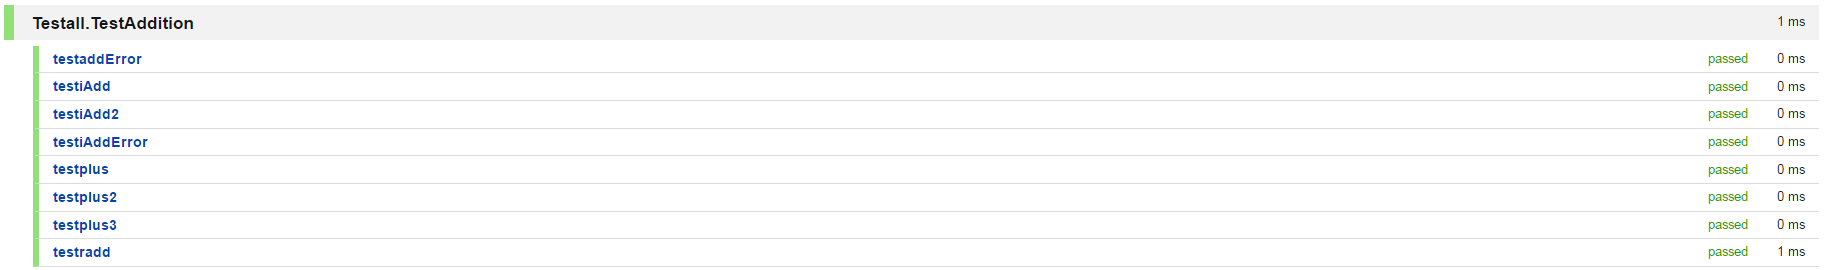
\includegraphics[width=1.1\linewidth]{images/testAddition}
\end{minipage}

\begin{minipage}{\linewidth}
	\centering
	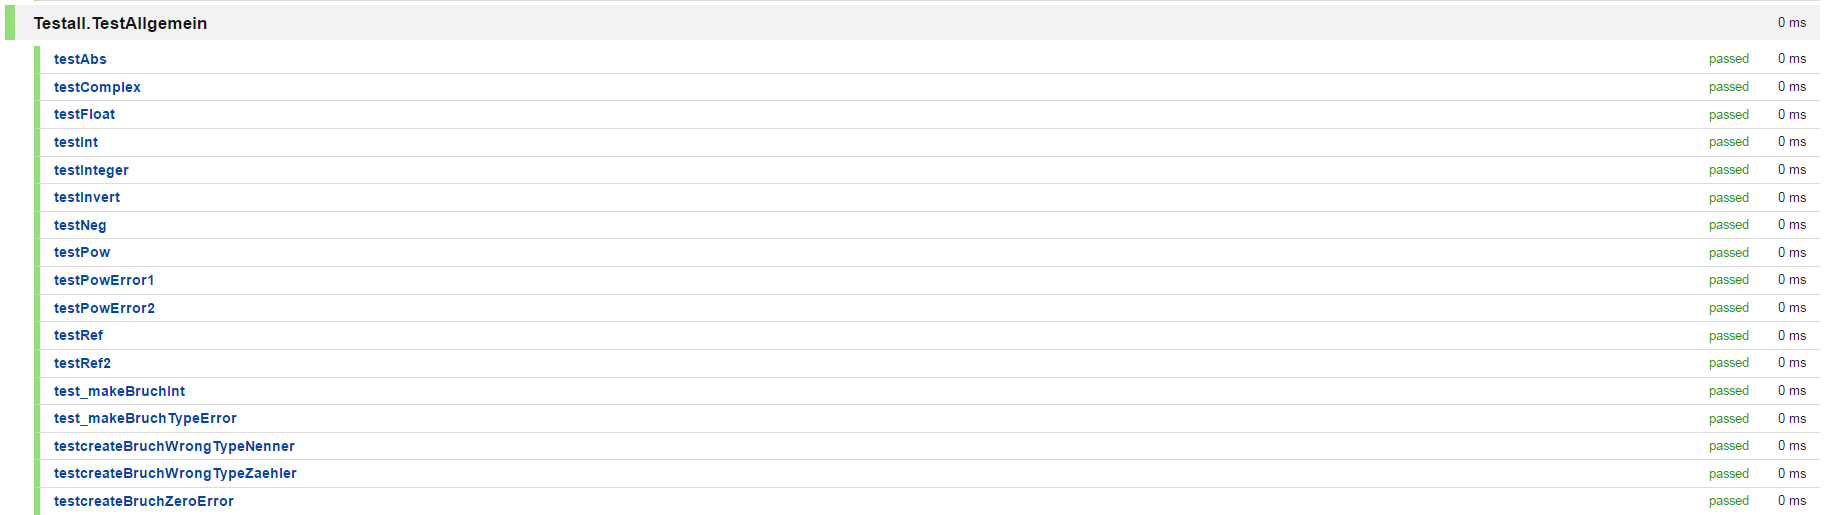
\includegraphics[width=1.1\linewidth]{images/testAllgemein}
\end{minipage}

\begin{minipage}{\linewidth}
	\centering
	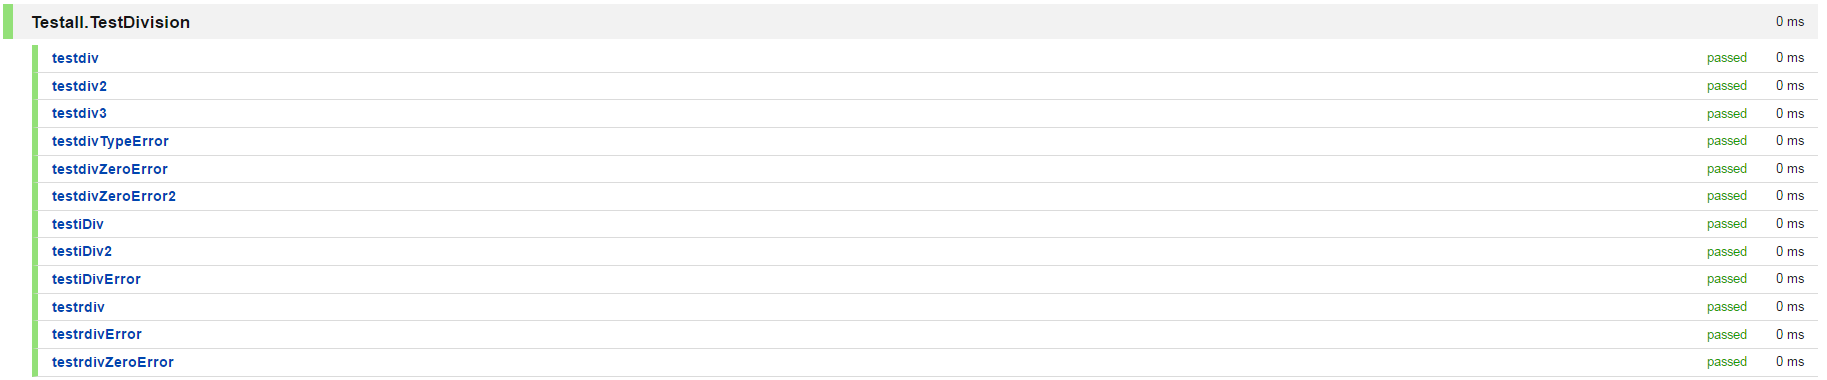
\includegraphics[width=1.1\linewidth]{images/testDivision}
\end{minipage}

\begin{minipage}{\linewidth}
	\centering
	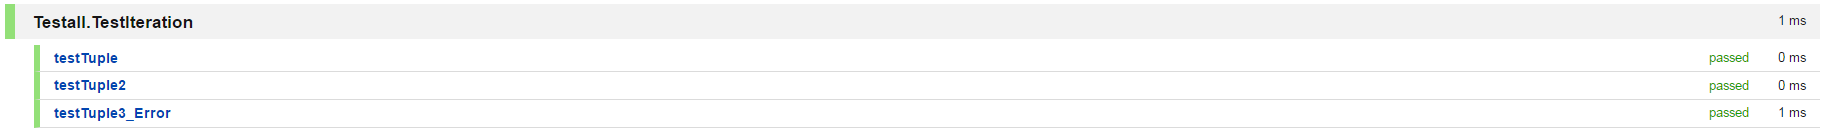
\includegraphics[width=1.1\linewidth]{images/testIteration}
\end{minipage}

\begin{minipage}{\linewidth}
	\centering
	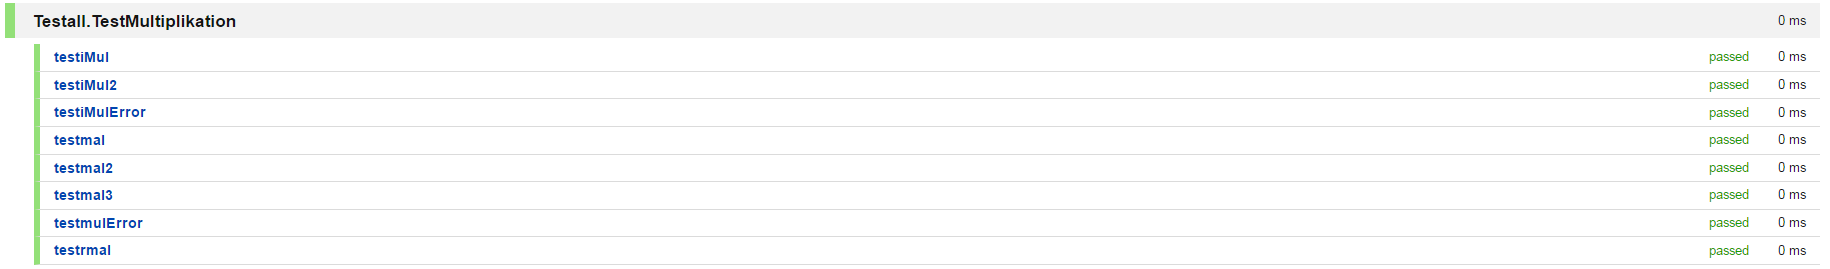
\includegraphics[width=1.1\linewidth]{images/testMultiplikation}
\end{minipage}

\begin{minipage}{\linewidth}
	\centering
	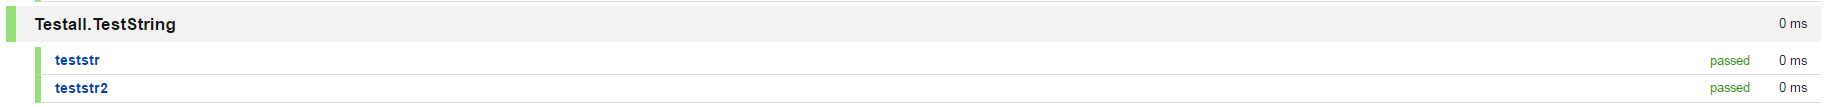
\includegraphics[width=1.1\linewidth]{images/testString}
\end{minipage}

\begin{minipage}{\linewidth}
	\centering
	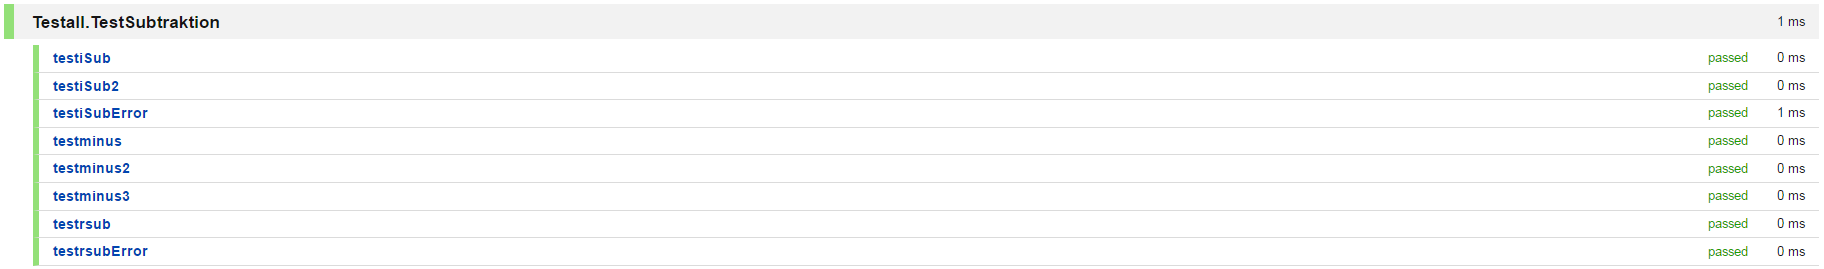
\includegraphics[width=1.1\linewidth]{images/testSubtraktion}
\end{minipage}

\begin{minipage}{\linewidth}
	\centering
	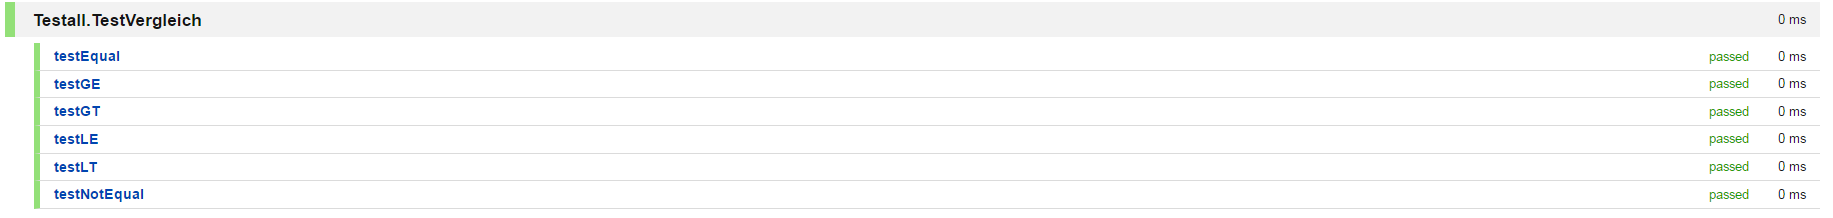
\includegraphics[width=1.1\linewidth]{images/testVergleich}
\end{minipage}

\subsection{Dokumentation}

\begin{minipage}{\linewidth}
	\centering
	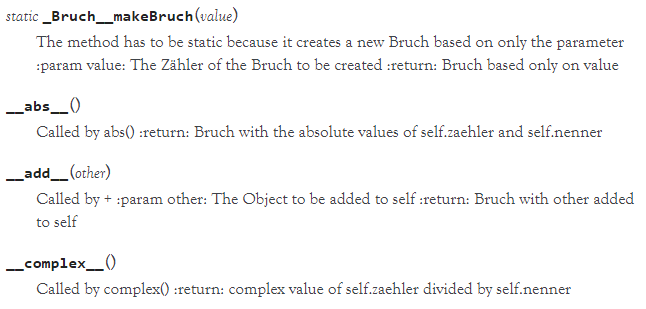
\includegraphics[width=1\linewidth]{images/dokumentation1}
\end{minipage}

\begin{minipage}{\linewidth}
	\centering
	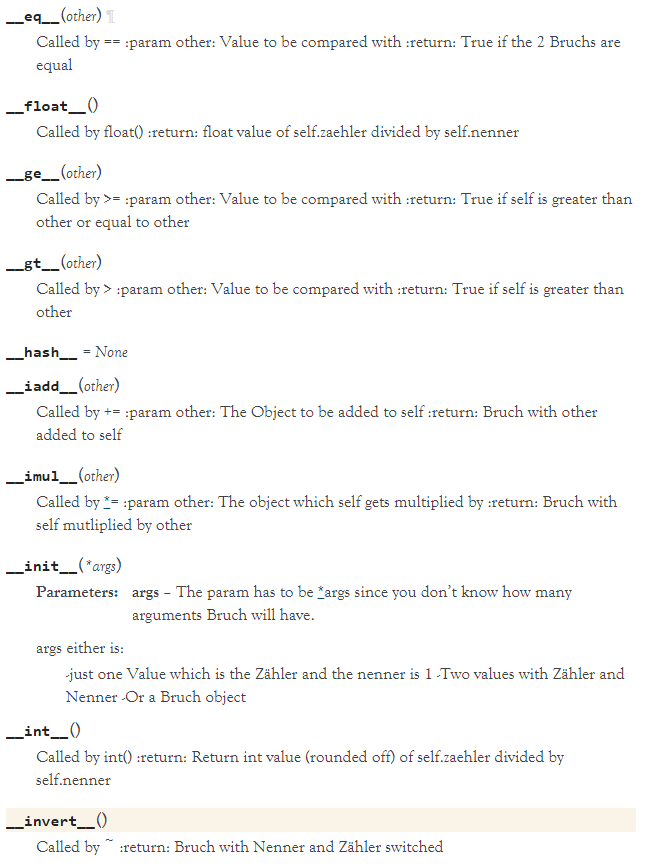
\includegraphics[width=1\linewidth]{images/dokumentation2}
\end{minipage}

\begin{minipage}{\linewidth}
	\centering
	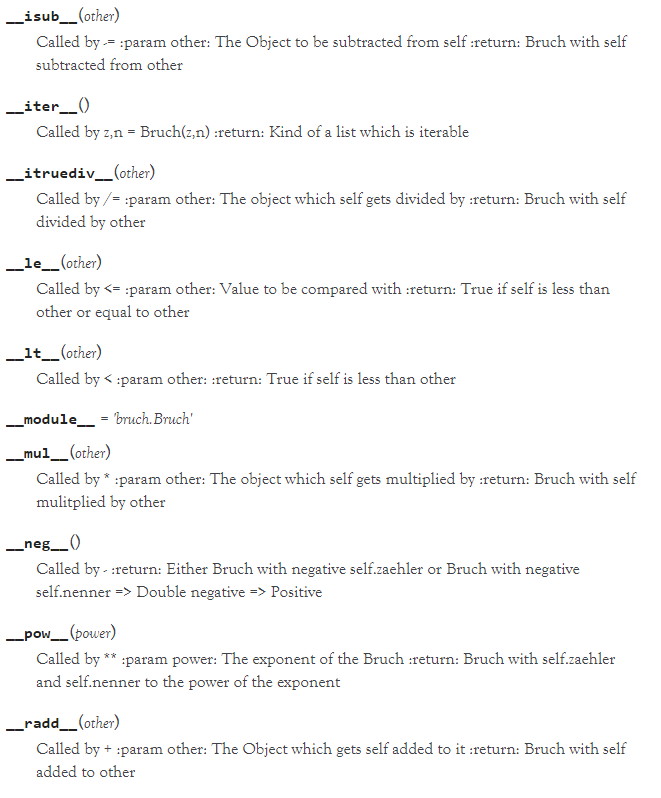
\includegraphics[width=1\linewidth]{images/dokumentation3}
\end{minipage}

\begin{minipage}{\linewidth}
	\centering
	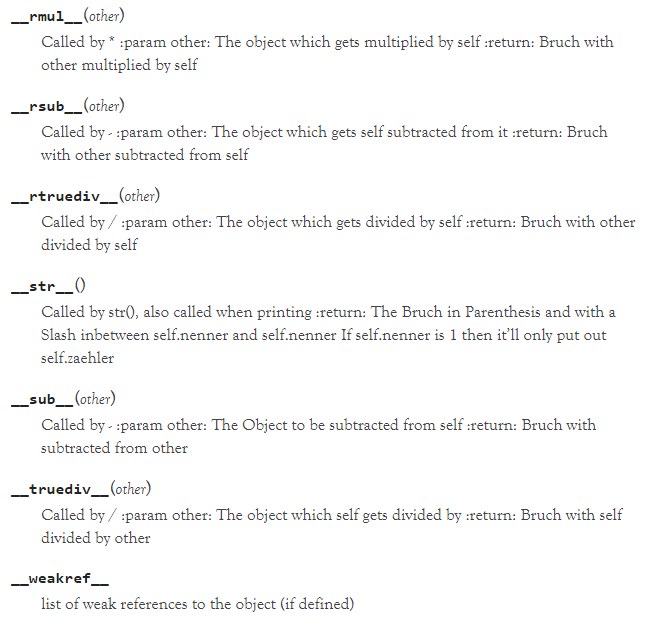
\includegraphics[width=1\linewidth]{images/dokumentation4}
\end{minipage}

\subsection{Github}
Die Implementation und Genaue Dokumentation ist auf meinem Github-Repository online gestellt:

\hyperlink{https://github.com/mwoelfer-tgm/Bruch}{https://github.com/mwoelfer-tgm/Bruch}